\documentclass{article}
\usepackage{graphicx} % Required for inserting images

\title{Labwork 3: Logistic Regression}
\author{Phi Doan Minh Luong - 24400464}
\date{May 2025}

\begin{document}

\maketitle

\setlength\parindent{0pt}

\section{Implementation}
- First, we implement functions to calculate the loss of all data points, and 3 partial derivatives over $w_0$, $w_1$, and $w_2$

- Read the csv file and extract the value of x and y as lists of floats

- Perform gradient descent to optimize the weights $w_0$, $w_1$, and $w_2$. It iteratively updates $w_0$, $w_1$, and $w_2$ using the gradients (df0, df1, and df2) and the learning rate $lr$

- After training, the optimized weights $w_0$, $w_1$, and $w_2$ are used to plot the regression line based on the learned weights, and a plot shows the loss over iterations

- Here is the result when the gradient descent is run for 10,000 iterations with a learning rate of 0.1 when the initial value for $w_0$, $w_1$, and $w_2$ is 0, 1, and 2 respectively
\begin{center}
    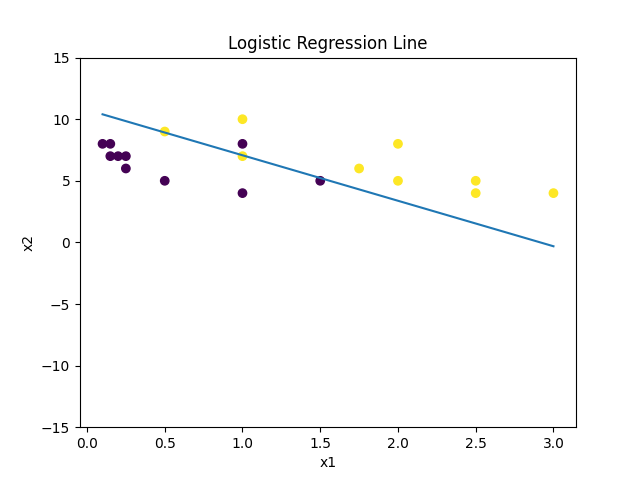
\includegraphics[width=0.5\linewidth]{1.png}
    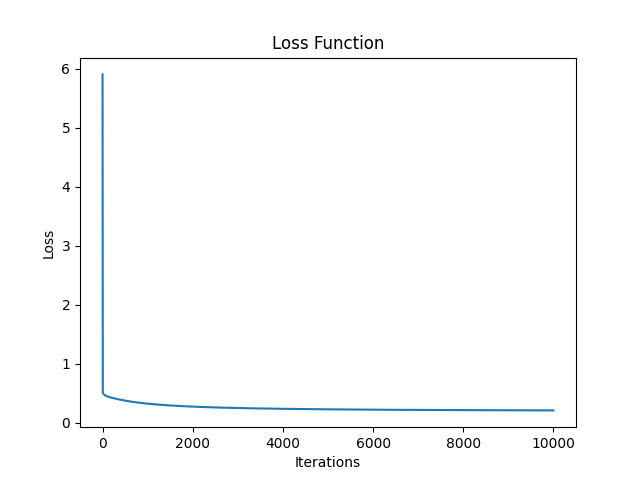
\includegraphics[width=0.5\linewidth]{2.png}
\end{center}

- After updating, the loss is around 0.21

\section{The effect of different learning rates for convergence}
\subsection{Learning rate is too small (0.0001)}
- When the learning rate is too small, it requires many updates before reaching the minimum point
\begin{center}
    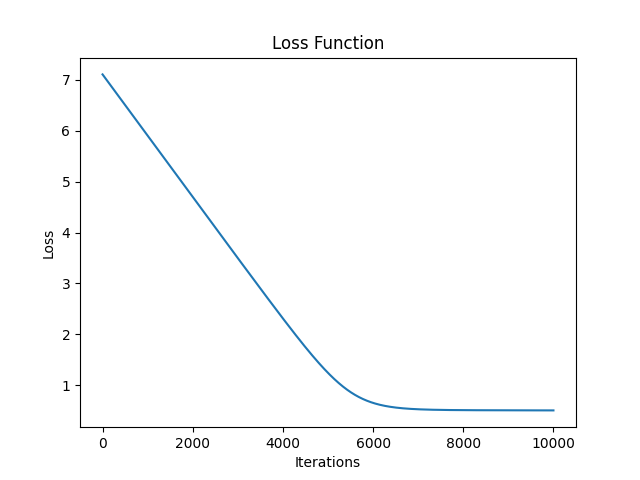
\includegraphics[width=0.5\linewidth]{3.png}
\end{center}

\subsection{Learning rate is too large (0.9)}
- When the learning rate is too large, it could cause drastic updates, which lead to divergent behaviors
\begin{center}
    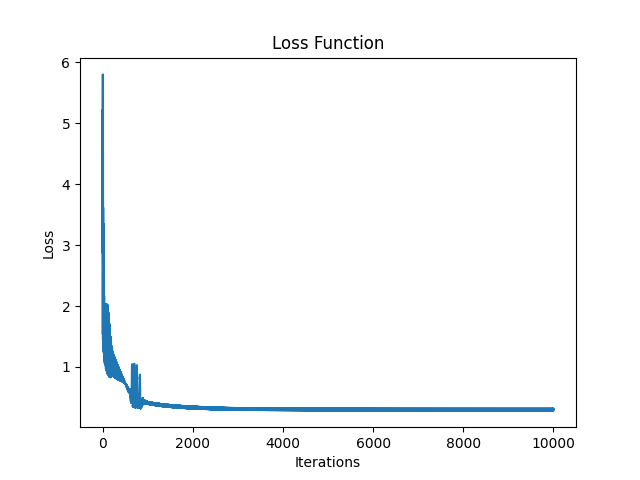
\includegraphics[width=0.5\linewidth]{4.png}
\end{center}
\end{document}
